\documentclass[a4paper]{article}
\usepackage[english]{babel}
\usepackage[utf8]{inputenc}
\usepackage{textcomp}
\usepackage{amsmath}
\usepackage{gensymb}
\usepackage{physics}
\usepackage{graphicx}
\usepackage[colorinlistoftodos]{todonotes}
\usepackage{xcolor}
\usepackage{array}
\usepackage{tabularx}
\usepackage{tikz}
\usepackage{framed}
\usepackage{xfrac}
\usepackage[most]{tcolorbox}
\usepackage{fix-cm}
\usepackage[margin=0.5in]{geometry}
\usetikzlibrary{quotes,angles}
\usetikzlibrary{decorations.pathreplacing}
\usetikzlibrary{calc}

\let\phi\varphi
\let\bf\textbf
\colorlet{shadecolor}{orange!15}
\newcommand\der[2]{\frac{d #1}{d #2}}
\def\centerarc[#1](#2)(#3:#4:#5){\draw[#1] ($(#2)+({#5*cos(#3)},{#5*sin(#3)})$) arc (#3:#4:#5)}
% Syntax: [draw options] (center) (initial angle:final angle:radius);

\title{Fixed-Axis Rotation}
\author{OpenStax University Physics Vol. 1}
\date{}

\begin{document}
\setcounter{section}{10}
\maketitle
\subsection{Rotational Variables}
\noindent\bf{Angular Velocity}
\vspace{2mm}\\
Uniform circular motion is motion in a circle at constant speed, although this is the simplest case of rotational motion, it is used here to introduce rotational variables.\par
The figure shows a particle moving in a circle. Its position vector from the origin of the circle to the particle sweeps out the angle $\theta$, which increases in the counterclockwise direction as the particle moves along its path. The angle $\theta$ is called the angular position of the particle. As the particle moves, it traces an arc length $s$.
\begin{center}
    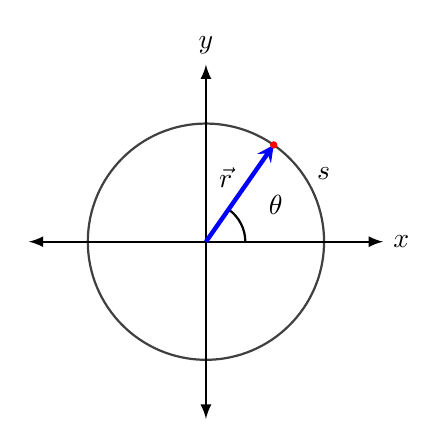
\begin{tikzpicture}[scale=1.5]
        %%% COORDINATES %%%
        \draw (0,0) coordinate (o);
        \draw ({cos(55)},{sin(55)}) coordinate (a);
        \draw ({cos(55)},0) coordinate (b);

        %%% AXES & CIRCLE %%%
        \draw[thick,draw=black!75] (0,0) circle (1);
        \draw[<->,thick,-latex] (0,0)--(1.5,0) node[right]{$x$};
        \draw[<->,thick,-latex] (0,0)--(0,1.5) node[above]{$y$};
        \draw[<->,thick,-latex] (0,0)--(-1.5,0);
        \draw[<->,thick,-latex] (0,0)--(0,-1.5);

        %%% POSITION VECTOR & ANGLE %%%
        \draw pic["$\theta$",draw=black,thick,-,angle eccentricity=2,angle radius=0.5cm]{angle=b--o--a};
        \draw[->,ultra thick,draw=blue,-stealth] (0,0)--node[left,xshift=0.5mm,yshift=2mm]{$\vec{r}$}({cos(55)},{sin(55)});

        \centerarc[red,very thick](0,0)(0:55:1);
        \node at ({1.15*cos(30)},{1.15*sin(30)}){$s$};
        \filldraw[red] ({cos(55)},{sin(55)}) circle (0.75pt);
    \end{tikzpicture}
\end{center}
The angle is related to the radius of the circle and the arc length by 
\begin{equation}
    \theta = \frac{s}{r}
\end{equation}
The angle $\theta$, the angular position of the particle moving along its path has units of radians (rad). As the particle moves along its circular path, its angular position changes and it undergoes angular displacements $\Delta\theta$.\par\vspace{1mm}
\noindent We can assign vectors to the quantities in equation 1, the angle $\vec{\theta}$ is a vector out of the page. The angular position vector $\vec{r}$ and the arc length vector $\vec{s}$ both lie in the plane of the page, they are related by:
\begin{equation}
    \vec{s} = \vec{\theta} \times \vec{r}
\end{equation}
The arc length is the cross product of the angle vector and the position vector
\begin{center}
    \begin{tikzpicture}[scale=2]
        \draw[->,-latex] (0,0)--(1,0) node[right]{$y$};
        \draw[->,-latex] (0,0)--(0,1) node[above]{$z$};
        \draw[->,-latex] (0,0)--(-{cos(45)},-{sin(45)}) node[left]{$x$};

        \draw[->,very thick,-stealth] (0,0)--node[right]{$\vec{\theta}$}(0,0.75);
        \draw[->,very thick,-stealth] (0,0)--node[below,xshift=-2mm,yshift=0.5mm]{$\vec{r}$}({0.7*cos(65)},{-0.7*cos(65)});
        \draw[->,very thick,-stealth,draw=red] ({0.7*cos(65)},{-0.7*cos(65)})--node[right,yshift=-1mm,xshift=-0.5mm]{$\vec{s}$}({0.7*cos(65) + 0.28},{-0.7*cos(65) + 0.28});
    \end{tikzpicture}
\end{center}
The magnitude of the angular velocity, denoted by $\omega$, is the time rate of change of the angle $\theta$ as the particle moves in a circular path. The instantaneous angular velocity, defined as the limit as $\Delta t \to 0$ of the average angular velocity $\bar{\omega} = \frac{\Delta\theta}{\Delta t}$
\begin{equation}
    \omega = \lim\limits_{\Delta t \to 0}\frac{\Delta\theta}{\Delta t} = \frac{d\theta}{dt}
\end{equation}
Where $\theta$ is the angle of rotation. The units of angular velocity are radians per second (rad\;s$^{-1}$). Angular velocity can also be referred to as the rotation rate in radians per second. In many cases, rotation rate is given in revolutions/s or cycles/s, to find angular velocity, multiply revolutions/s by $2\pi$ (since there are $2\pi$ radians per revolution). Since a positive angle in a circle is counterclockwise, we take counterclockwise rotations as being positive and clockwise rotations as negative.\vspace{1mm}\par
\noindent We can see how angular velocity is related to the tangential speed of the particle by differentiating equation 1 with respect to time. Equation 1 can be rewritten as:
\begin{align*}
    s = \theta r
\end{align*}
\newpage
\noindent Taking the derivative with respect to time and noting that the radius $r$ is constant gives:
\begin{align*}
    \der{s}{t} = \der{}{t}(r\theta) = \theta\der{r}{t} + r\der{\theta}{t} = r\der{\theta}{t}
\end{align*}
Where $\theta\der{r}{t} = 0$. Here, $\der{s}{t}$ is just the tangential speed $v_t$ of the particle moving in a circular path. Using equation 3 we arrive at:
\begin{equation}
    v_t = r\omega
\end{equation}
The tangential speed of the particle is its angular velocity times the radius of the circle. The tangential speed of the particle increases with its distance from the axis of rotation for a constant angular velocity. The figure shows two particles placed at different radii on a rotating disk with constant angular velocity. As it rotates, the tangential speed increases linearly with the radius from the axis of rotation. We see that $v_1 = r_1\omega_1$ and $v_2 = r_2\omega_2$. The disk has a constant angular velocity so $\omega_1 = \omega_2$. This means that $\frac{v_1}{r_1} = \frac{v_2}{r_2}$ or $v_2 = \big(\frac{r_2}{r_1}\big)$. Thus, since $r_2 > r_1$, $v_2 > v_1$
\begin{center}
    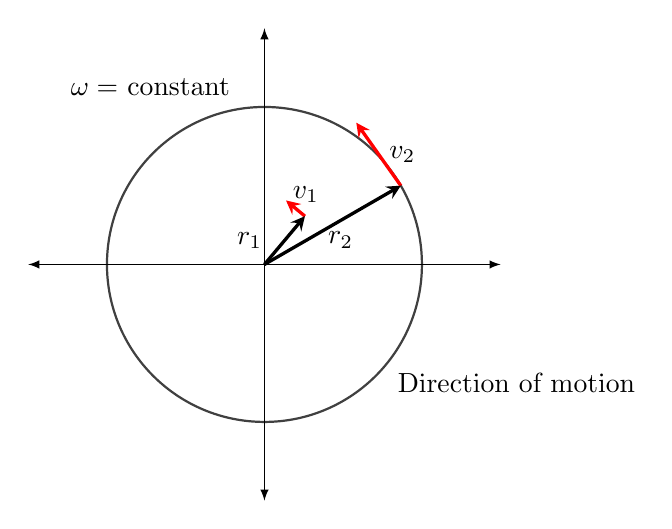
\begin{tikzpicture}[scale=2]
        %%% COORDINATES %%%
        \draw (0,0) coordinate (O);
        \draw ({cos(30)},{sin(30)}) coordinate (a);
        \draw ({0.4*cos(50)},{0.4*sin(50)}) coordinate (b);

        %%% AXES & CIRCLE %%%
        \draw[thick,draw=black!75] (0,0) circle (1);
        \draw[->,-latex] (O)--(1.5,0);
        \draw[->,-latex] (O)--(-1.5,0);
        \draw[->,-latex] (O)--(0,1.5);
        \draw[->,-latex] (O)--(0,-1.5);

        %%% LINES %%%
        \draw[->,very thick,-stealth,draw=red] (a)--node[right]{$v_2$}({cos(30) - 0.4*cos(45)},{sin(30) + 0.4});
        \draw[->,very thick,-stealth,draw=red] (b)--({0.4*cos(50) - 0.17*cos(45)},{0.4*sin(50) + 0.1}) node[right,yshift=0.75mm,xshift=-0.5mm]{$v_1$};
        \draw[->,very thick,-stealth] (O)--node[below,xshift=1mm,yshift=0.5mm]{$r_2$}(a);
        \draw[->,very thick,-stealth] (O)--node[left,xshift=-1.5mm]{$r_1$}(b);

        \node at ({-1.45*cos(60)},{1.3*sin(60)}){$\omega =$ constant};

        \centerarc[->,black!50,thick,-stealth](0,0)(-30:-10:1.1);
        \centerarc[->,black!50,thick,-stealth](0,0)(60:80:1.1);
        \centerarc[->,black!50,thick,-stealth](0,0)(150:170:1.1);
        \centerarc[->,black!50,thick,-stealth](0,0)(240:260:1.1);
        \node at (1.6,-0.75){Direction of motion};
    \end{tikzpicture}
\end{center}
Similar to equation 2, one can state a cross product relation to the vector of the tangential velocity as stated in equation 4, therefore:
\begin{equation}
    \vec{v} = \vec{\omega} \times \vec{r}
\end{equation}
The tangential velocity is the cross product of the angular velocity and the position vector as shown below. On the left we see that with the angular velocity in the $+z$ direction, the rotation in the $xy$ plane is counterclockwise. On the right, the angular velocity is in the $-z$ direction, which gives a clockwise rotation in the $xy$ plane.
\begin{center}
    \begin{tikzpicture}[scale=2]
        \draw[->,-latex] (0,0)--(1,0) node[right]{$y$};
        \draw[->,-latex] (0,0)--(0,1) node[above]{$z$};
        \draw[->,-latex] (0,0)--(-{cos(45)},-{sin(45)}) node[left]{$x$};

        \draw[->,very thick,-stealth] (0,0)--node[right]{$\vec{\omega}$}(0,0.75);
        \draw[->,very thick,-stealth,draw=red] ({0.7*cos(65)},{-0.7*cos(65)})--node[right,yshift=-1mm,xshift=-0.5mm]{$\vec{v}$}({0.7*cos(65) + 0.26},{-0.7*cos(65) + 0.26});
        \draw[->,very thick,-stealth] (0,0)--node[below,xshift=-2mm,yshift=0.5mm]{$\vec{r}$}({0.7*cos(65)},{-0.7*cos(65)});
    \end{tikzpicture}
    \hspace{15mm}
    \begin{tikzpicture}[scale=2]
        \draw[->,-latex] (0,0)--(1,0) node[right]{$y$};
        \draw[->,-latex] (0,0)--(0,1) node[above]{$z$};
        \draw[->,-latex] (0,0)--(-{cos(45)},-{sin(45)}) node[left]{$x$};

        \draw[->,very thick,-stealth] (0,0)--node[left]{$\vec{\omega}$}(0,-0.75);
        \draw[->,very thick,-stealth,draw=red] ({0.7*cos(65)},{-0.7*cos(65)})--node[right,yshift=-1mm,xshift=-0.5mm]{$\vec{v}$}({0.7*cos(65) - 0.26},{-0.7*cos(65) - 0.26});
        \draw[->,very thick,-stealth] (0,0)--node[above,yshift=-1.5mm,xshift=1.5mm]{$\vec{r}$}({0.7*cos(65)},{-0.7*cos(65)});
    \end{tikzpicture}
\end{center}
\begin{shaded}
    \underline{\bf{Example 10.1:} Rotation of a Flywheel}
    \vspace{2mm}\\
    A flywheel rotates such that it sweeps out an angle at the rate of $\theta = \omega t = (45.0\text{ rad\;s}^{-1})t$ radians. The wheel rotates counterclockwise when viewed in the plane of the page.
    \begin{enumerate}
        \item[(a)] What is the angular velocity $\omega$ of the flywheel?
        \vspace{1mm}\\
        $\displaystyle \omega = \der{\theta}{t} = 45$ rad\;s$^{-1}$, angular velocity is constant
        \item[(b)] What direction is the angular velocity?
        \vspace{1mm}\\
        The direction of rotation is counterclockwise, so the direction of angular velocity is $+z$
        \item[(c)] How many radians does the flywheel rotate through in 30 s?
        \vspace{1mm}\\
        $\displaystyle \theta(t) = \omega t \to \Delta\theta = \theta(30$ s$) - \theta(0$ s$) = \theta(30$ s$) \to (45.0$ rad\;s$^{-1})(30$ s$) = 1350.0$ rad
        \item[(d)] What is the tangential speed of a point on the flywheel 10 cm from the axis of rotation
        \vspace{1mm}\\
        $v_t = r\omega = (0.1$ m$)(45.0$ rad\;s$^{-1}) = 4.5$ ms$^{-1}$
    \end{enumerate}
\end{shaded}
\newpage
\noindent\bf{Angular Acceleration}
\vspace{2mm}\\
For describing situations where $\omega$ changes, we need to define angular acceleration. The faster the change in $\omega$, the greater the angular acceleration. Instantaneous angular acceleration $\alpha$ is defined as the derivative of angular velocity with respect to time:
\begin{equation}
    \alpha = \lim_{\Delta t \to 0}\frac{\Delta\omega}{\Delta t} = \der{\omega}{t} = \frac{d^2\theta}{dt^2}
\end{equation}
Where we have taken the limit of the average angular acceleration $\bar{\alpha} = \frac{\Delta\omega}{\Delta t}$ as $\Delta t \to 0$. The units of angular acceleration are radians/s per second, or rad\;s$^{-2}$. 
\vspace{1mm}\par
\noindent In the same way that the vector associated with angular velocity $\vec{\omega}$ was defined, we can define $\vec{\alpha}$, the vector associated with angular acceleration. If the angular velocity is along the $+z$ axis and $\der{\omega}{t}$ is positive, the angular acceleration $\vec{\alpha}$ is positive and points along the $+z$ axis, if $\der{\omega}{t}$ is negative, the angular acceleration is negative and points along the $-z$ axis.

\begin{center}
    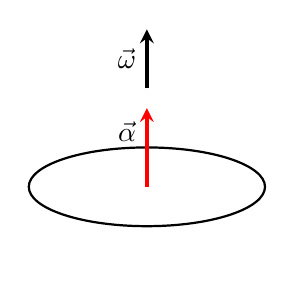
\begin{tikzpicture}
        \draw[thick] (0,0) ellipse (1.5 and 0.5);
        \draw (0,0) coordinate (O);
        \draw[->,very thick,-stealth,draw=red] (O)--node[left,yshift=2mm]{$\vec{\alpha}$}(0,1);
        \draw[->,very thick,-stealth] (0,1.25)--node[left]{$\vec{\omega}$}(0,2);
        \centerarc[->,black!50,thick,-stealth](0,0)(-10:10:1.7);
        \node at (0,-1){};
    \end{tikzpicture}
    \hspace{15mm}
    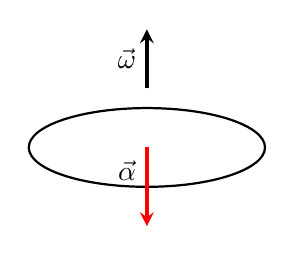
\begin{tikzpicture}
        \draw[thick] (0,0) ellipse (1.5 and 0.5);
        \draw (0,0) coordinate (O);
        \draw[->,very thick,-stealth,draw=red] (O)--node[left,yshift=2mm]{$\vec{\alpha}$}(0,-1);
        \draw[->,very thick,-stealth] (0,0.75)--node[left]{$\vec{\omega}$}(0,1.5);
        \centerarc[->,black!50,thick,-stealth](0,0)(-10:10:1.7);
    \end{tikzpicture}
\end{center}
The tangential acceleration vector can be expressed as a cross product of the angular acceleration and position vectors. This equation can be found by taking the derivative of equation 5
\begin{equation}
    \vec{a} = \vec{\alpha} \times \vec{r}
\end{equation}
The vector relationships for angular acceleration and tangential acceleration are shown below
\begin{center}
    \begin{tikzpicture}[scale=2]
        \draw[->,-latex] (0,0)--(1,0) node[right]{$y$};
        \draw[->,-latex] (0,0)--(0,1) node[above]{$z$};
        \draw[->,-latex] (0,0)--(-{cos(45)},-{sin(45)}) node[left]{$x$};

        \draw[->,very thick,-stealth] (0,0)--node[right]{$\vec{\alpha}$}(0,0.75);
        \draw[->,very thick,-stealth,draw=red] ({0.7*cos(65)},{-0.7*cos(65)})--node[right,yshift=-1mm,xshift=-0.5mm]{$\vec{a}$}({0.7*cos(65) + 0.26},{-0.7*cos(65) + 0.26});
        \draw[->,very thick,-stealth] (0,0)--node[below,xshift=-2mm,yshift=0.5mm]{$\vec{r}$}({0.7*cos(65)},{-0.7*cos(65)});
    \end{tikzpicture}
    \hspace{15mm}
    \begin{tikzpicture}[scale=2]
        \draw[->,-latex] (0,0)--(1,0) node[right]{$y$};
        \draw[->,-latex] (0,0)--(0,1) node[above]{$z$};
        \draw[->,-latex] (0,0)--(-{cos(45)},-{sin(45)}) node[left]{$x$};

        \draw[->,very thick,-stealth] (0,0)--node[left]{$\vec{\alpha}$}(0,-0.75);
        \draw[->,very thick,-stealth,draw=red] ({0.7*cos(65)},{-0.7*cos(65)})--node[right,yshift=-1mm,xshift=-0.5mm]{$\vec{a}$}({0.7*cos(65) - 0.26},{-0.7*cos(65) - 0.26});
        \draw[->,very thick,-stealth] (0,0)--node[above,yshift=-1.5mm,xshift=1.5mm]{$\vec{r}$}({0.7*cos(65)},{-0.7*cos(65)});
    \end{tikzpicture}
\end{center}
Tangential acceleration of a point on a rotating body at a distance from the axis of rotation can be related in the same way as tangential velocity and angular velocity. Differentiating equation 4 with respect to time (the radius $r$ is constant) gives:
\begin{equation}
    a_t = r\alpha
\end{equation}
The tangential acceleration $a_t$ is the radius times the angular acceleration
\begin{shaded}
    \underline{\bf{Example 10.2:} A Spinning Bike Wheel}
    \vspace{2mm}\\
    A bicycle mechanic mounts a bicycle on the repair stand and starts the rear wheel spinning from rest to a final angular velocity of 250 rpm in 5.00 s.
    \begin{enumerate}
        \item[(a)] Calculate the average angular acceleration in rad\;s$^{-2}$
        \begin{align*}
            \displaystyle \bar{\alpha} = \frac{\Delta\omega}{\Delta t} = \frac{250\text{ rpm}}{5.00\text{ s}}
        \end{align*}
        Converting from rpm to rad\;s$^{-1}$:
        \begin{align*}
            \Delta\omega = 250\frac{\text{rev}}{\text{min}} \cdot \frac{2\pi\text{ rad}}{\text{rev}} \cdot \frac{1\text{ min}}{60\text{ s}} = 26.2\text{rad\;s}^{-1}
        \end{align*}
        Entering this back into the expression for $\alpha$ gives:
        \begin{align*}
            \alpha = \frac{\Delta\omega}{\Delta t} = \frac{26.2\text{ rad\;s}^{-1}}{5.00\text{ s}} = 5.24\text{ rad\;s}^{-2}
        \end{align*}
        \item[(b)] If the brakes are hit, causing an angular acceleration of -87 rad\;s$^{-2}$, how long does it take the wheel to stop?
        \vspace{1mm}\\
        Angular velocity decreases from 26.2 rad\;s$^{-1}$ to zero so $\Delta\omega = -26.2$ rad\;s$^{-1}$, and $\alpha$ is given to be -87.3 rad\;s$^{-2}$
        \begin{align*}
            \Delta t = \frac{\Delta\omega}{\alpha} = \frac{-26.2\text{ rad\;s}^{-1}}{-87.3\text{ rad\;s}^{-2}} = 0.300\text{ s}
        \end{align*}
    \end{enumerate}
\end{shaded}

\newpage
\begin{shaded}
    \underline{\bf{Example 10.3:} Wind Turbine}
    \vspace{2mm}\\
    A wind turbine in a wind farm is being shut down for maintenance. It takes 30 s for the turbine to go from its operating angular velocity to a complete stop in which the angular velocity function is $\omega(t) = \Big[\frac{(t\text{s}^{-1} - 30.0)^2}{100.0}\Big]$rad\;s$^{-1}$, where $t$ is the time in seconds. If the turbine is rotating counterclockwise looking into the page:
    \begin{enumerate}
        \item[(a)] What are the directions of the angular velocity and acceleration vectors?
        \vspace{1mm}\\
        Since the turbine is rotating counterclockwise, angular velocity $\vec{\omega}$ points towards $+z$. Since the angular velocity is decreasing, the angular acceleration $\vec{\alpha}$ points towards $-z$
        \item[(b)] What is the average angular acceleration?
        \vspace{1mm}\\
        At $t = 0$, the initial angular velocity of the turbine is $\omega = 9.0$ rad\;s$^{-1}$, the final angular velocity is zero, so the average angular velocity $\bar{\alpha}$ is:
        \begin{align*}
            \bar{\alpha} = \frac{\Delta\omega}{\Delta t} = \frac{\omega - \omega_0}{t - t_0} = \frac{0 - 9.0\text{ rad\;s}^{-1}}{30.0 - 0\text{ s}} = -0.3\text{ rad\;s}^{-2}
        \end{align*}
        \item[(c)] What is the instantaneous angular acceleration at $t = 0.0, 15.0, 30.0$ s?
        \vspace{1mm}\\
        Taking the derivative of angular velocity with respect to time gives
        \begin{align*}
            \alpha = \der{\omega}{t} = \bigg[\frac{(t - 30.0)}{50.0}\bigg]\text{ rad\;s}^{-2}
        \end{align*}
        Thus:\hspace{2.5mm} $\alpha(0.0\text{ s}) = -0.6$ rad\;s$^{-2}$, $\alpha(15.0\text{ s}) = -0.3$ rad\;s$^{-2}$, and $\alpha(30.0\text{s}) = 0$ rad\;s$^{-2}$
    \end{enumerate}
\end{shaded}

\end{document}